\documentclass{article}

\textwidth=150mm
\textheight=220mm
\topmargin=0pt
\headheight=0pt
\oddsidemargin=7mm
\headsep=0pt

\newcommand*{\sm}[1]{$\scriptstyle #1$}

\usepackage{tikz}
\usetikzlibrary{positioning,through,calc,intersections,arrows.meta,external}
\tikzset{>=stealth} % Use stealth arrows

\begin{document}
\thispagestyle{empty}
\begin{center}

\vspace{10ex}

\textbf{\huge Surprising Geometric Constructions}

\vspace{10ex}


\hspace*{9pt}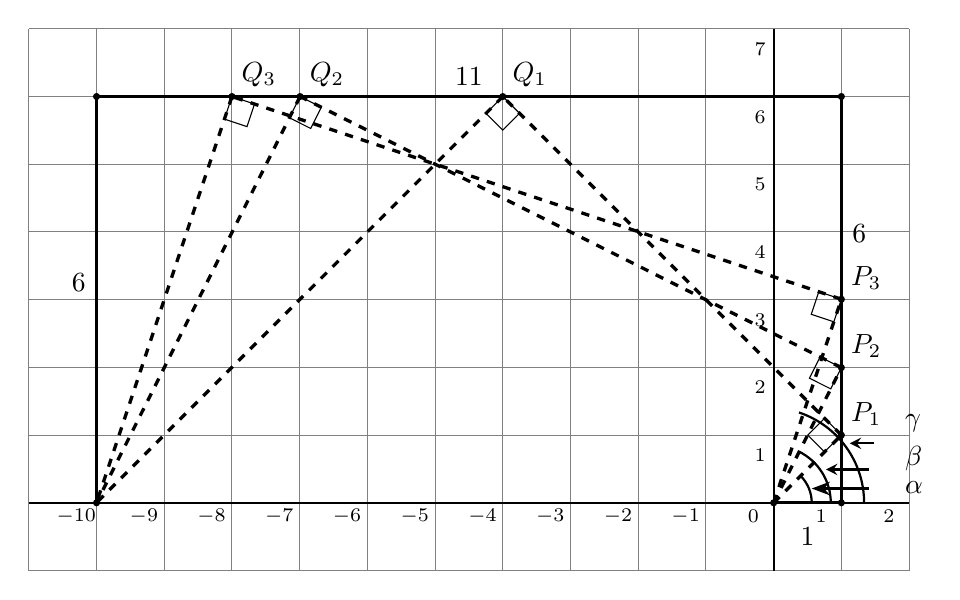
\begin{tikzpicture}[scale=.86]
% Draw help lines and axes
\draw[step=10mm,white!50!black] (-11,-1) grid (2,7);
\draw[thick] (-11,0) -- (2,0);
\draw[thick] (0,-1) -- (0,7);
\foreach \x in {-10,...,2}
  \node at (\x-.3,-.2) {\sm{\x}};
\foreach \y in {1,...,7}
  \node at (-.2,\y-.3) {\sm{\y}};
\coordinate (A) at (0,0);
\coordinate (B) at (1,0);
\coordinate (C) at (1,6);
\coordinate (D) at (-10,6);
\coordinate (E) at (-10,0);
\foreach \x in {A,B,C,D,E}
  \fill (\x) circle(1.5pt);
\draw[very thick] (A) --
  node[below,yshift=-5pt] {$1$} (B);
\draw[very thick,name path=bc] (B) -- 
  node[right,yshift=24pt] {$6$} (C);
\draw[very thick,name path=cd] (C) --
  node[above] {$11$}(D);
\path[name path=de] (D) -- ($(E)+(0,-.8)$);
\draw[very thick] (D) --
  node[left,yshift=6pt] {$6$} (E);


% Draw first segment of first second path
\path[name path=a1] (A) -- +(45:3);
\path [name intersections = {of = a1 and bc, by = {A1}}];
\fill (A1) circle(1.5pt) node[above right] {$P_1$};
\draw[very thick,dashed] (A) -- (A1);
\draw[thick] ($(A) + (16pt,0)$)
  arc [start angle=0, end angle = 45, radius=16pt];
\node[above right,xshift=44pt,yshift=0pt] at (A) {$\alpha$};
\draw[rotate=135] (A1) rectangle +(10pt,10pt);
\draw[Stealth-,thick] ($(A) + (16pt,6pt)$) -- +(24pt,0);

% Draw second segment of first second path
\path[name path=b1] (A1) -- +(135:8);
\path [name intersections = {of = b1 and cd, by = {B1}}];
\fill (B1) circle(1.5pt) node[above right] {$Q_1$};
\draw[very thick,dashed] (A1) -- (B1);
\draw[rotate=225] (B1) rectangle +(10pt,10pt);

% Draw third segment of first second path
\draw[very thick,dashed] (B1) -- (E);

% Draw first segment of second second path
\path[name path=a2] (A) -- +(63.4:4);
\path [name intersections = {of = a2 and bc, by = {A2}}];
\fill (A2) circle(1.5pt) node[above right] {$P_2$};
\draw[very thick,dashed] (A) -- (A2);
\draw[thick] ($(A) + (24pt,0)$)
  arc [start angle=0, end angle = 63.4, radius=24pt];
\node[above right,xshift=44pt,yshift=8pt] at (A) {$\beta$};
\draw[rotate=153.4] (A2) rectangle +(10pt,10pt);
\draw[<-,thick] ($(A) + (22pt,14pt)$) -- +(18pt,0);

% Draw second segment of second second path%
\path[name path=b2] (A2) -- +(153.4:10);
\path [name intersections = {of = b2 and cd, by = {B2}}];
\fill (B2) circle(1.5pt) node[above right] {$Q_2$};
\draw[very thick,dashed] (A2) -- (B2);
\draw[rotate=243.4] (B2) rectangle +(10pt,10pt);

% Draw third segment of second second path%
\draw[very thick,dashed] (B2) -- (E);

% Draw first segment of second second path%
\path[name path=a3] (A) -- +(71.6:4);
\path [name intersections = {of = a3 and bc, by = {A3}}];
\fill (A3) circle(1.5pt) node[above right] {$P_3$};
\draw[very thick,dashed] (A) -- (A3);
\draw[thick] ($(A) + (38pt,0)$)
  arc [start angle=0, end angle = 71.6, radius=40pt];
\node[above right,xshift=44pt,yshift=22pt] at (A) {$\gamma$};
\draw[rotate=161.6] (A3) rectangle +(10pt,10pt);
\draw[<-,thick] ($(A) + (32pt,25pt)$) -- +(10pt,0);

% Draw second segment of second second path%
\path[name path=b3] (A3) -- +(161.6:10);
\path [name intersections = {of = b3 and cd, by = {B3}}];
\fill (B3) circle(1.5pt) node[above right] {$Q_3$};
\draw[very thick,dashed] (A3) -- (B3);
\draw[rotate=251.6] (B3) rectangle +(10pt,10pt);

% Draw third segment of second second path%
\draw[very thick,dashed] (B3) -- (E);
\end{tikzpicture}

\vspace{6ex}

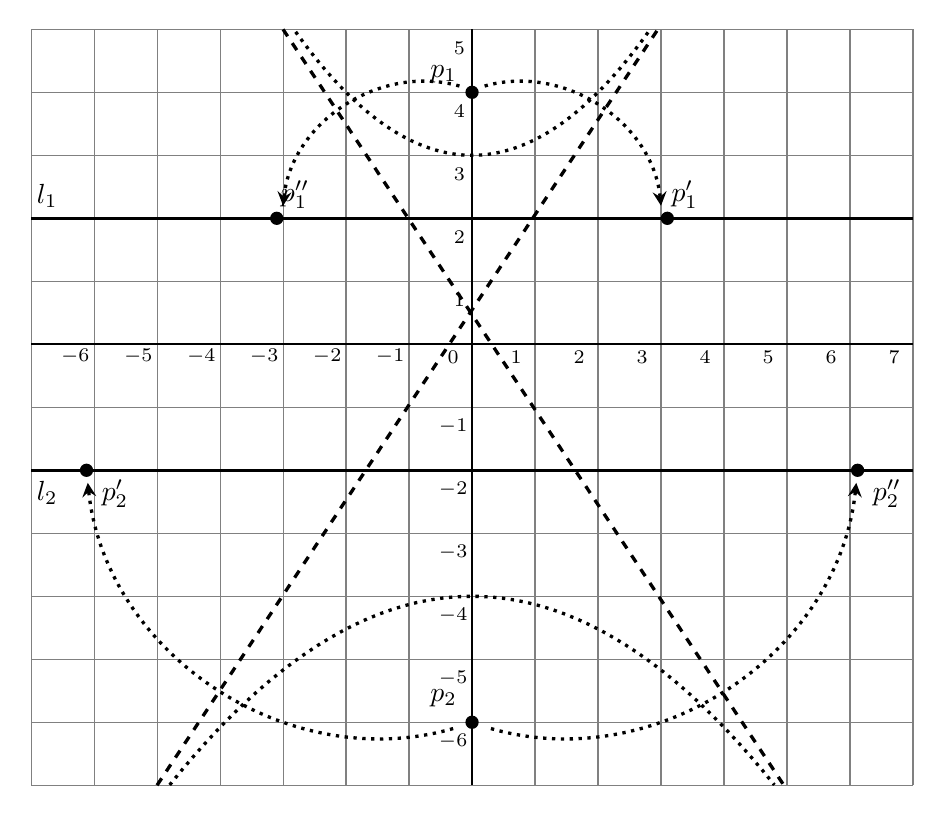
\begin{tikzpicture}[scale=.8]
\draw[step=10mm,white!50!black,thin] (-7,-7) grid (7,5);
\draw[thick] (-7,0) -- (7,0);
\draw[thick] (0,-7) -- (0,5);
\foreach \x in {-6,...,7}
  \node at (\x-.3,-.2) {\sm{\x}};
\foreach \y in {1,...,5}
  \node at (-.2,\y-.3) {\sm{\y}};
\foreach \y in {-6,...,-1}
  \node at (-.3,\y-.3) {\sm{\y}};
  
\coordinate (P1) at (0,4);
\fill (P1) circle (3pt) node[above left,xshift=-2pt] {$p_1$};
\coordinate (P2) at (0,-6);
\fill (P2) circle (3pt) node[above left,xshift=-2pt,yshift=2pt] {$p_2$};

\coordinate (P1P) at (3.1,2);
\fill (P1P) circle (3pt) node[above right,xshift=-2pt] {$p_1'$};
\coordinate (P2P) at (-6.12,-2);
\fill (P2P) circle (3pt) node[below right,xshift=2pt] {$p_2'$};

\coordinate (P1PP) at (-3.1,2);
\fill (P1PP) circle (3pt) node[above right,xshift=-2pt] {$p_1''$};
\coordinate (P2PP) at (6.12,-2);
\fill (P2PP) circle (3pt) node[below right,xshift=2pt] {$p_2''$};

\draw[very thick] (-7,2) -- node[very near start,above,xshift=-34pt] {$l_1$} (7,2);
\draw[very thick] (-7,-2) -- node[very near start,below,xshift=-34pt] {$l_2$} (7,-2);

\draw[domain=-4.8:4.8,samples=50,very thick,dotted] plot (\x,{-.13*\x*\x-4});
\draw[domain=-2.8:2.8,samples=50,very thick,dotted] plot (\x,{.25*\x*\x+3});

\draw[very thick,dashed] (-5,-7) -- (2.95,5);
\draw[very thick,dashed] (-3,5) -- (4.95,-7);

\draw[very thick,dotted,->,bend left=50] (.2,4.1) to (3,2.2);
\draw[very thick,dotted,->,bend left=50] (-.3,-6.1) to (-6.1,-2.2);

\draw[very thick,dotted,->,bend right=50] (-.2,4.1) to (-3,2.2);
\draw[very thick,dotted,->,bend right=50] (.3,-6.1) to (6.1,-2.2);
\end{tikzpicture}

\vspace{10ex}

\textbf{\LARGE Moti Ben-Ari}

\end{center}
\end{document}
